\documentclass{msuphddissertation}
\usepackage{amsmath}
\usepackage{amsfonts}
\usepackage{graphicx}
%\usepackage{hyperref}
\usepackage{enumitem}
\usepackage{minibox}
\usepackage{color}
\usepackage{siunitx}\sisetup{per-mode=symbol}
%\usepackage{tabularx}
\usepackage{listings}

%
%	FRONT
%

\author{Michael J. Obsniuk}
\title{Identifying Computational Practices in Introductory Physics}
\unit{Physics --- Doctor of Philosophy}

\begin{document}

\maketitlepage

\begin{abstract}
\end{abstract}

\TOC
\LOT
\LOF

\newpage
\pagenumbering{arabic}
\begin{doublespace}

%
%	INTRODUCTION (VERY HIGH LEVEL)
%

\chapter{Introduction}

Starting in the 1960's and continuing to present day, computers continue to revolutionize the way that we do and teach science.  They play an increasingly integral role in everyday life.  From their ability to analyze large sets of data to their ability to model chaotic physical systems, modern computers are powerful and useful tools.  Given the implications this tool has on modern scientific research (e.g., modeling biological or social systems), it has become of national level importance\cite{AAPT2016}.

Computation is important not only in terms of modern research in professional domains, but also as a pedagogical tool in educational domains.  In order for an individual to develop professional computational skills, he must practice them -- and there is no better place to practice than in an introductory physics course.  Obviously, the particular skills an individual will need to be proficient in will depend on the particular job.  However, focusing on the general practices that students should engage in while solving complex engineering and science problems is a reasonable place to start.

Accordingly, Secs.~\ref{} and \ref{} will focus on computation's utility in both research and pedagogy, respectively.  We will then introduce computational thinking in Sec.~\ref{} and the computational practices that accompany it in Sec.~\ref{}.  With these introductory ideas,  we can begin to buttress our study.

\section{As a research tool}

Computation is increasingly being referred to as the third leg of modern physics, along with experiment and theory.  Its utility in solving complicated problems (e.g., predicting chaotic or non-linear motion) that cannot currently be solved analytically makes it indispensable in many field, from physics to chemistry to biology to engineering.

% A description of predictive motion and Euler-Cromer update.  Could also mention Runge-Kutte and MANY OTHER styles that all have the same basic form: numerically solving complicated differential equations. 

\section{As a pedagogical tool}

%	Add in a description of Easy Java Simulations.  

Sherwood developed and maintained VPython until it turned in Glowscript.  VPython was expressly designed to engage students with computational modeling and the three-dimensional visualization that are characteristic to it.

Chabay et al. have studied computation involving VPython in introductory physics classrooms from a number of different lenses.  These lenses range from investigating difficulties that students run into while computationally modeling, to investigating how to be incorporate computation into the classroom, to investigating how students are thinking computationally.

Although much work has been done around computation at the introductory level, there are still many unanswered or only partially answered questions.  Answering these questions requires a deep understanding of the types of thinking and practices that students are engaging in while computing.  Accordingly, we must introduce computational thinking and the accompanying computational practices.

\section{Computational thinking}

Computational thinking is a term that has become increasingly popular since its introduction in the early 1980s.  This term, although frequently used today, is difficult to concisely explain given its many and varied definitions.  Even within the fields of education and computer science, many different viewpoints exist on the topic, and the corresponding definitions are just as varied \cite{Grover2013}.  However, many of these definitions share one fundamental characteristic: solving complex problems through abstraction and analytic thinking with the aid of computer algorithms.

Seymour Papert first introduced computational thinking in terms of students actively constructing knowledge (constructionism) through the production of an artifact (i.e., a computer program).  However, Papert does not initially attempt to define computational thinking.  Rather, he comments that attempts to integrate computational thinking into everyday life have failed because of the insufficient definition of computational thinking.  He optimistically claims that more attempts to define computational thinking will be made and eventually the ``pieces will come together \cite{Papert1981}.''  Papert would later go on to say that computational thinking involves ``forging new ideas'' that are both ``accessible and powerful \cite{Papert1996}.''

Building on Papert, Jeanette Wing defines computational thinking in terms of taking advantage of the processing power of modern computers with the addition of human creativity.  This echoes the core sentiments expressed by Papert: Using human creativity to forge new ideas that are computationally powerful.  Wing is careful to remind readers that computational thinking is a fundamental skill for everyone, not just computer scientists \cite{Wing2008}.

Further elaboration by Alfred Aho points out that the process of finding the right tool for the right job is a clear indicator of computational thinking.  Mathematical abstraction (modeling) is at the heart of computational thinking, and be able to choose between competing abstractions (models) is of critical importance \cite{Aho2012}.  Aho points out that although there are many useful definitions of computational thinking within computer science, new domains of investigation (e.g., introductory physics) require definitions of their own.

Most recently, the Next Generation Science Standards (NGSS) laid out a framework for identifying computational thinking in K-12 settings.  As early as the fifth grade students are expected to be able to think computationally.  They describe computational thinking, at this level, in terms of analyzing data and comparing approaches.  By the time students reach middle school, computational thinking advances to analyzing large data sets and generating explanations.  Finally, in high school, computational thinking expands to constructing computational models and using them to answer questions \cite{NGSS2012}.  Clearly, computational thinking is a complicated concept which requires substantial explanation.

Experts in the field still have a ways to go when it comes to clearly defining computational thinking within physics education.  However defined, though, this type of abstract and algorithmic thinking is pervasive -- it extends beyond computer science into fields from geology to astronomy, and even beyond STEM \cite{Bundy2007}.  It is becoming increasingly clear that ``computational thinking is a fundamental skill for everyone, not just computer scientists \cite{Wing2006}.''

One such domain of investigation that could benefit from a clear definition of computational thinking is that of introductory physics.  Many realistic physics problems require thinking abstractly and the computational power of computers (i.e., non-linear forces in Newton's second law).  This combination of abstract and algorithmic thinking (computational thinking) is the ``heart'' of the ``computational physics approach'' to solving problems \cite{AAPT2016}.  This approach relies heavily on computational thinking as it relates to a particular tool and on both technical and physics computational skills.  The AAPT defines 3 technical skills and 7 physics skills.

Many of the physics skills defined by the AAPT involve modeling and the modeling process.  Computational modeling is a powerful problem solving tool.  Research shows that computational modeling can be successfully incorporated into the (middle-divison) physics classroom \cite{Caballero2011}.  There are a number of common mistakes students make when solving a Newtonian gravitational problem.  We should encourage students to synthesize both analytic and computational skills \cite{Caballero2014,MORE}

Other research on (high school) computational modeling has focused on success.  Students' ability to adapt to novel problems seems to rest on the ability to synthesize physics and computational skills \cite{Aiken2012}.  The ability of students to understand the iterative process, that is characteristic of computation, plays a crucial role in the ability to construct novel computational force models.

To summarize, research shows that computational thinking is desirable in many fields and still lacks precise defintion.  Also, it shows that adding computation and computational thinking to a course is difficult and there are many mistakes that need to be worried about by instructors.  Additionally, it shows that the iteration that is characteristic of physics and computational thinking is linked to the ability to adapt to novel problems.  Therefore, it is important to encourage computational thinking in introductory physics courses.

\section{Computational physics practices}

The efficient construction of domain specific knowledge by students has always been one of the ultimate goals of physics education research.  The fundamental concepts, ideas, and theories of introductory physics are the foundation for all inquiry in not just the field of physics, but in many related disciplines (e.g., chemistry and engineering).  However, there is more to being a productive member of the scientific community than just amassing a collection of facts -- it is important that this knowledge be applied in some practical way (e.g., utilizing Newton's second law to numerically predict the trajectory of a rocket).  For this reason, the NGSS has broadly defined scientific practices as a combination of both knowledge and skill ``to emphasize that engaging in scientific investigation requires not only skill but also knowledge that is specific to each practice \cite{NGSS2013}.''

Given the recent interest in scientific practices, and computational thinking more specifically, a taxonomy of the computational practices indicative of computational thinking has been defined \cite{Weintrop2015}.  This taxonomy, comprised of twenty-two individual yet inter-related practices, fitting into four different categories, is meant to help guide instructors and researchers as they attempt to teach and better understand computational thinking in science classrooms.  Each practice, according to the taxonomy, is defined broadly so as to be applicable to a wide range of science classrooms.

However, the broad definitions that make the taxonomy widely applicable also leave it relatively vague and difficult to apply to any particular situation.  Reducing the vagueness and difficulty of applying this taxonomy to a specific domain of inquiry (i.e., introductory physics) is a challenging but important task.  Having a taxonomy that is both precise and easy to apply will provide a solid foundation for instructors to generate/validate computational problems and for researchers to analyze the learning process.  Accordingly, it is important that we identify, through direct observation, the set of computational practices that are common to computational introductory physics.  This involves not only identifying the practices, but also the underlying knowledge and skills.

In Ch.~\ref{ch:background} we explicate the prior research on computation and its results, as well as the theoretical and methodological underpinnings of the study.  This includes the historical and recent results from Physics Education Research (PER) and Computer Science Education Research (CSER).  In Ch.~\ref{ch:context}, we describe the course from which our data has been collected -- a calculus-based introductory physics course with a focus on engineering, working in groups, and computation.  We also describe the types of computational problems students are working on in class.  In Ch.~\ref{ch:motivation}, we provide a motivation for not only the existence of the study, but also the theories and methods that we decided on using.  Our theories and methodologies used depended highly on the type of data that we had and the type of research we were conducting.  In Chs.~\ref{ch:analysis}--\ref{ch:conclusion}, we present the analysis and results of our current study with concluding remarks.

%
%	BACKGROUND (VERY DETAILED)
%

\chapter{Background} %	VERY DETAILED

\section{Historical and Recent comp. research}

Chabay et. al.

Expand on computational research here.

\section{Methods for my research}

Thematic analysis.

\section{Framework}

AAPT and Weintrop.

Provide a table for the AAPT and Weintrop practices.

%
%	CONTEXT (P3)
%

\chapter{Context}

It is important to understand the course from which we have collected our data to better understand the results of our study.  That course -- called Projects and Practices in Physics (${\rm P}^{3}$) -- is based on a social constructivist theory of learning and a flipped/problem-based pedagogy.  In other words, students familiarize themselves with relevant material before coming to class, where they will work in small groups to actively and socially construct knowledge while solving complex analytical and computational physics and engineering problems.  The course has intentionally been designed to encourage computational thinking wherever possible.  Specifically, computational thinking has been incorporated into the notes, pre- and post-class homework, in-class feedback and assessments, and a selection of the in-class problems.

\section{Course design}

Each week in ${\rm P}^{3}$, students are expected to do a number of things. They must read and complete the pre-class homework based on information gathered from the pre-class notes.  They must work in small groups on two related analytical problems or a mixture of one related analytical and one related computational problem during the two two-hour weekly meetings.  For the computational problem, that means designing and constructing a correct computational force model in a small group and answering follow-up questions.  There are also post-class homework questions based on information gathered from the pre-class notes and the in-class problems.  This all occurs while students simultaneously prepare for the following week.

%For example, in the third week of the semester, the pre-class notes and homework focus on this and that.  The analytic problem is this, and the computational problem is that.  The computational practices students must engage with are this, and the tutor questions look like this.  The feedback that students receive often encourages computational practices like this.  The post-class homework focuses on this.

\section{Introduction to VPython}

Given that the vast majority of students enter ${\rm P}^{3}$ with little to no prior programming experience, we need to ensure that they are prepared to handle computational problems early in the semester.  One way that we can achieve this is by requiring students to engage with the fundamental programming ideas before coming to class through pre-class homework and notes.  These notes and homework questions highlight the fundamental physical and programming ideas specific to VPython and the computational problems that will be delivered in class.

For example, consider the portion of the course notes shown in Fig.~\ref{}.  These notes are made available to the students at the beginning of the semester.  The content is meant to provide students with a basic understanding of the utility of VPython and a list of common errors.

\begin{figure}[ht]\centering
%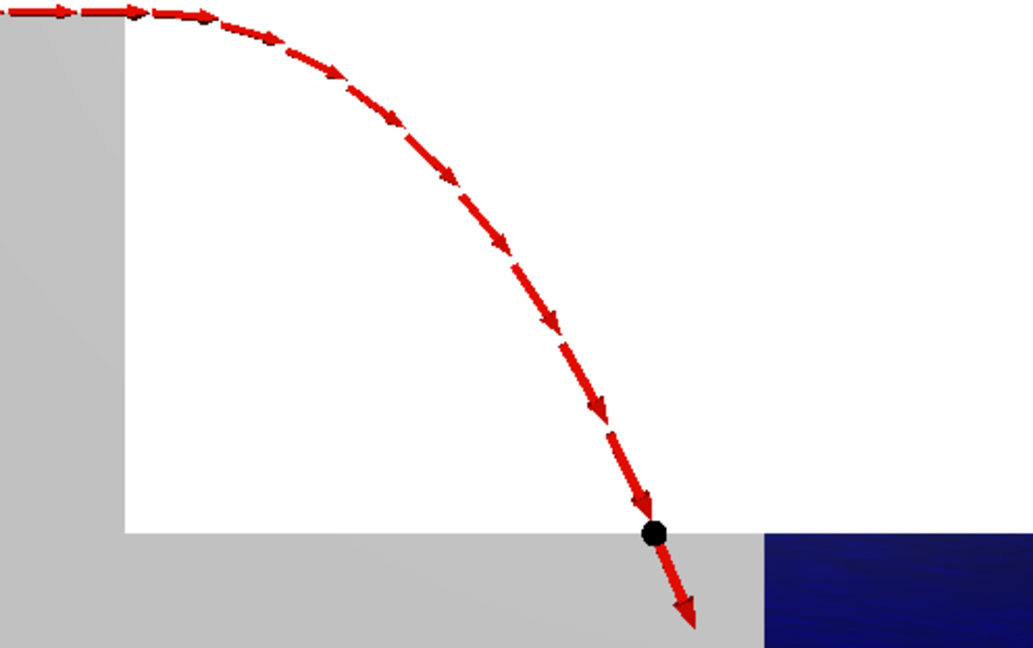
\includegraphics[scale=1]{images/visual.pdf}
\caption{Page of on-line notes introducing computional physics.  The picture is just a placeholder.}
\end{figure} 

\section{Pre-class work}

Similarly, consider the pre-class homework questions shown in Fig.~\ref{} that are made available at the beginning of the third week of the course.  This question is meant to demonstrate that there are multiple correct ways that a unit vector can be constructed in code.  Given the nature of the corresponding week's computational problem (see Sec.~\ref{}), we expect students to be able to draw on and take advantage of this knowledge when faced with a related albeit more complicated problem.

\begin{figure}[ht]\centering
%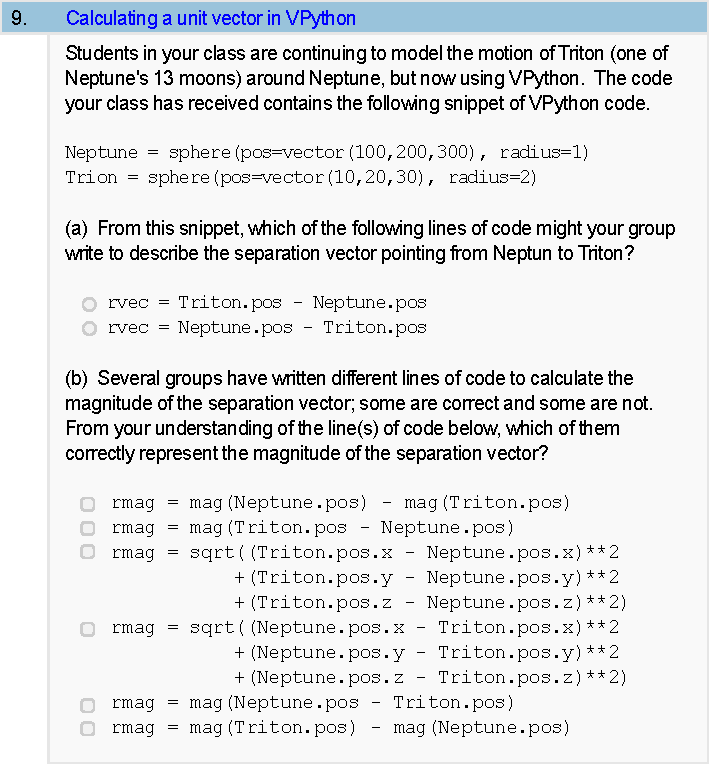
\includegraphics[scale=1]{images/comphw.pdf}
\caption{Pre-class homework question focusing on the different ways that the magnitude of a vector can be constructed in VPython code.}
\end{figure} 

\section{In-class tasks}

\begin{figure}[ht]\centering
%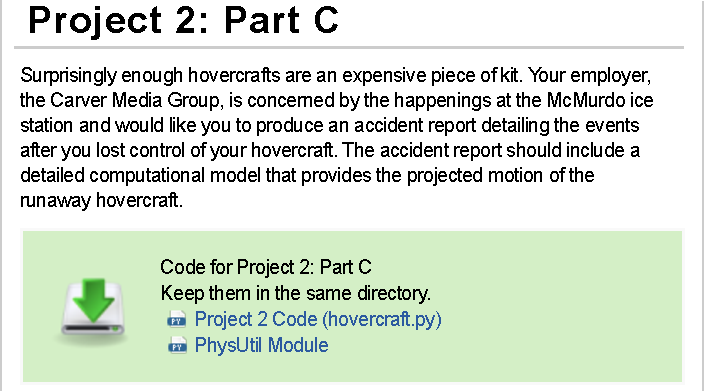
\includegraphics[scale=1]{images/partc.pdf}
\caption{A schedule for the semester.  The images is just a placeholder.}
\end{figure}

There are a number of in-class computational problems spread out throughout the semester (see Fig.~\ref{}).  The first few computational problems focus on different force models and the resulting linear motion of objects.  The last few computational problems focus on extended objects and their rotation.  While solving these problems, groups are expected to engage in a number of computational practices that the problems have been designed around: \begin{enumerate}
\item[P1.] developing and using models,
\item[P2.] planning and carrying out investigations,
\item[P3.] analyzing and interpreting data,
\item[P4.] using mathematics and computational thinking,
\item[P6.] constructing explanations,
\item[P7.] and engaging in argument from evidence.
\item[P8.] and obtaining, evaluating, and communicating information.
\end{enumerate}

One of the scientific practices used heavily on both analytic and computation days is that of (P1) developing and using models.  Whether those models be mathematical or computational, we expect students to not only work together in groups to develop the model, but also to utilize that model in further investigations.  This type of scientific practice (P1) and the associated learning goals\cite{Irving2017} were further used to generate the type of in-class project that this study focuses on.

\subsection{Analytic problem}

\subsection{Computational problem}

This study focuses on the third and most complicated computational problem delivered to the students, shown in both Figs.~\ref{} and ~\ref{}. In order to focus our analysis on specific challenges students demonstrate while working this problem, we developed a framework for analyzing this problem by performing an expert task analysis on the problem.  A task analysis consists of breaking a complex ``task'' (e.g., modeling a gravitational system) down into related ``sub-tasks'' (e.g., determine the direction of the force). We aim to identify somewhat more manageable steps that must be taken in order to complete the overall task \cite{catra}.

The task analysis of this problem was initially constructed by a single content expert. After the first iteration it was presented to additional experts. Through this discussion, it became clear that the construction of the position dependent Newtonian gravitational force in code is a multi-step procedure involving a number of different sub-tasks. The task analysis was iteratively refined through this process until all experts agreed that the sub-tasks were sufficiently described to be useful in video analysis. At the same time, targeted pre-class homework problems were developed to help scaffold students overcoming what we perceived to be challenges based on the task analysis.  In doing so, we attempted to place (most) students in the Zone of Proximal Development (ZPD)\cite{vyg}. For example, the pre-class homework problems shown in Fig.~\ref{unit_hw} were developed to facilitate student understanding of the unit vector of a separation vector between two objects prior to working the computational problem.

\begin{table}[hb]\centering
\begin{tabular}{ll}
\textbf{Step (Sub-Task)} & \textbf{Associated Code} \\\hline
Construct separation vector & \begin{lstlisting}
sep = obj2.pos
\end{lstlisting}\\
between interacting objects & \begin{lstlisting}
         - obj1.pos
\end{lstlisting}\\\hline
Construct the unit vector & \begin{lstlisting}
usep = sep/mag(sep)
\end{lstlisting}\\\hline
Construct the net force & \begin{lstlisting}
Fnet = -G*m1*m2*usep
\end{lstlisting}\\
vector & \begin{lstlisting}
         /mag(sep)**2
\end{lstlisting}\\\hline
Integrate the net force over & \begin{lstlisting}
obj.p = obj.p + Fnet*dt
\end{lstlisting}\\
time into momentum & \\
\end{tabular}\caption{Some of the necessary steps that must be taken when constructing a Newtonian gravitational force in code.  Each step is associated with the construction/modification of a line of code.\label{tab1}}
\end{table}

With an agreed upon task analysis, we further focused our video analysis on the sub-tasks that were closely related to the construction of the position dependent Newtonian gravitational force (see Table.~\ref{tab1}).  In order to identify when groups were actually engaging in these sub-tasks, we analyzed groups on two levels: their \textit{speech}, including any and all words or utterances, and the associated \textit{visuals}, including any drawings, writings, lines of code, gestures, or simulation visualizations.  Theses two levels were then used to better understand how students overcome the challenges associated with the problem.

\begin{figure}[ht]\centering
%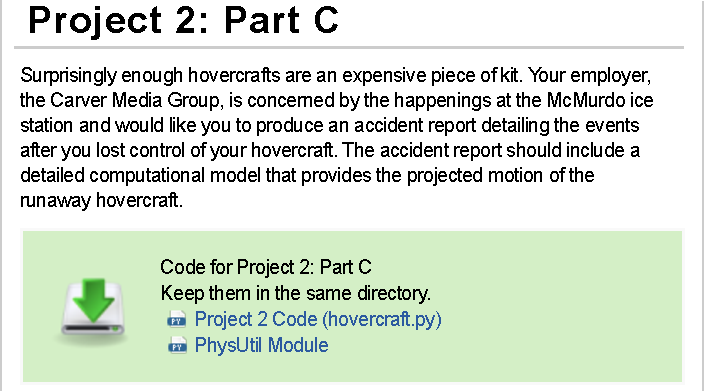
\includegraphics[scale=1]{images/partc.pdf}
\caption{In-class problem focusing on a non-constant net force model.  The picture is just a placeholder at this point.}
\end{figure}

\subsubsection{MWPs}

\subsubsection{TQs}

\subsection{Feedback/Assessment}

\subsection{Post-class work}

%
%	MOTIVATION
%

\chapter{Motivation}

Aside from a general interest in introductory computational physics, it is important to understand the underlying motivation(s) for the current study.

The process of identifying an interesting computational practice, described in Sec.~\ref{sec:debug}, was the earliest motivation for this study.  We found that it was extremely difficult to define and identify the particular practice of what we named ``physics debugging.''  Not only did the practice need to be clearly defined, it also needed to be clearly identified in the data.  This required a lot of in-depth qualitative analysis and inter-rater reliability, motivating our use of the Weintrop framework and the qualitative methods of Clarke in the current study.

Additionally, as described in Sec.~\ref{sec:phenom}, we found that it was very difficult to understand the qualitatively different ways in which students experienced computational introductory physics.  This difficulty motivated a task analysis with a focus on identifying practices that the students were engaging in through in-class observation, as opposed to their experiences through out-of-class interviews.
  
\section{Debugging}\label{sec:debug}

In this section, we present a case study of a group of students immersed in this ${\rm P}^{3}$ environment solving a computational problem.  This problem requires the translation of a number of fundamental physics principles into computer code.  Our analysis consists of qualitative observations in an attempt to describe, rather than generalize, the computational interactions, debugging strategies, and learning opportunities unique to this novel environment.

We focus this case study on the interactions between group and computer to begin to understand the ways in which computation can influence learning.  Particularly, we are interested in the interactions occurring simultaneously with social exchanges of fundamental physics principles (FPPs) specific to the present task (e.g., discussing $d\mathbf{r}=\mathbf{v}\,dt$ on a motion task) and the display of desirable problem solving strategies (e.g., divide-and-conquer).  These group-computer interactions vary in form, from the more active process of sifting through lines of code, to the more passive process of observing a three-dimensional visual display.

One previously defined computational interaction that reinforces desirable strategies,\cite{Murphy2008} borrowing from computer science education research, is the process of debugging.  Computer science defines debugging as a process that comes after testing \emph{syntactically} correct code where programmers ``find out exactly where the error is and how to fix it.''\cite{McCauley2008}  Given the generic nature of the application of computation in computer science environments (e.g., data sorting, poker statistics, or ``Hello, World!'' tasks), we expect to see unique strategies specific to a computational \emph{physics} environment.  Thus, we extend this notion of computer science debugging into a physics context to help uncover the strategies employed while groups of students debug \emph{fundamentally} correct code that produces unexpected physical results.

\subsection{Analysis}

In Fall 2014, ${\rm P}^{3}$ was run at Michigan State University in the Physics Department.  It was this first semester where we collected \emph{in situ} data using three sets of video camera, microphone, and laptop with screencasting software to document three different groups each week.  From the subset of this data containing computational problems, we \emph{purposefully sampled} a particularly interesting group in terms of their computational interactions, as identified by their instructor.  That is, we chose our case study not based on generalizability, but rather on the group's receptive and engaging nature with the project as an \emph{extreme case}.\cite{Flyvbjerg2006}

The project that the selected group worked on for this study consists of creating a computational model to simulate the geosynchronous orbit of a satellite around Earth.  In order to generate a simulation that produced the desired output, the group had to incorporate a position dependent Newtonian gravitational force and the update of momentum, using realistic numerical values.  The appropriate numerical values are Googleable, though instructors encouraged groups to solve for them analytically.

This study focuses on one group in the fourth week of class (the fourth computational problem seen) consisting of four individuals: Students A, B, C, and D.  The group had primary interaction with one assigned instructor.  Broadly, we see a 50/50 split on gender, with one ESL international student.  Student A had the most programming experience out of the group.  It is through the audiovisual and screencast documentation of this group's interaction with each other and with the technology available that we began our analysis.

To focus in on the group's successful physics debugging occurring over the $\SI{2}{\hour}$ class period, we needed to identify phases in time when the group had recognized and resolved a physics bug.  These two phases in time, \emph{bug recognition} and \emph{bug resolution} are the necessary limits on either side of the process of \emph{physics debugging}, as represented in Fig.~\ref{phases}.  We identified these two bounding phases at around $\SI{60(5)}{\minute}$ into the problem, and further examined the process of debugging in-between.  That is, we focused on the crucial moments surrounding the final modifications that took the code from producing unexpected output to expected output.

\begin{figure}\centering
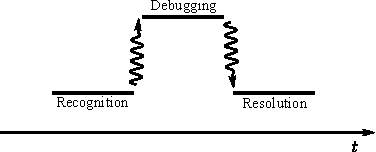
\includegraphics[scale=1]{./images/phases.pdf}
\caption{The debugging process necessarily corresponds to a phase beset on either side by the phases of recognition and resolution.  Note the absence of a vertical scale, as the vertical separation merely acts to distinguish phases.}
\end{figure}

\subsubsection{Recognition}

\subsubsection{Resolution}

\section{Phenomenography}\label{sec:phenom}

A description of the phenomenography study.

\subsection{Protocol}

A description of the development of the protocol.

\subsection{Analysis}

Since there are no real results, we can just describe how we analyzed the interview data.

%
%	ANALYSIS
%

\chapter{Analysis}

\section{Specific methods}

\section{Findings}

Recall that, according to the framework, each category of practice can be broken down into a number of individual practices.  Each individual practice, further, can be identified in terms of a number of fundamental characteristics.  Depending on the particular situation, some categories show up in the data more often than others.  For example, we expect to see fewer systems thinking practices and more computational modeling practices.  Further, within any category, some individual practices show up in the data more than others.  For example, within the data practices, we expect to see fewer instances of collecting data and more instances of creating data.

Most importantly, within any individual practice, there is a broad set of defining characteristics.  Ideally, each characteristic would be present in some form when its corresponding practice has been identified.  However, each characteristic can be organized in terms of being either necessary or sufficient for the cause.  That is, we need not necessarily observe every characteristic in order to identify a practice according to the framework.

\begin{figure}[ht]\centering
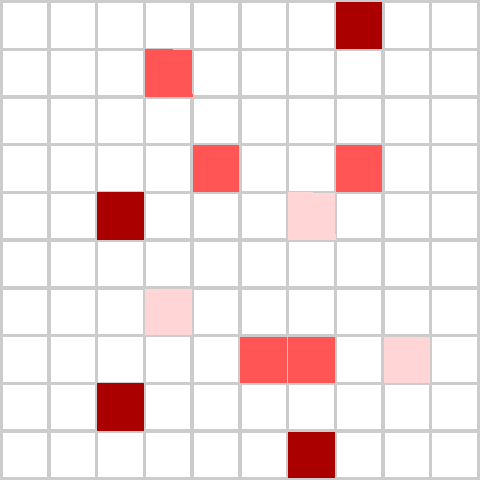
\includegraphics[scale=1]{./images/matrix.pdf}
\caption{A ``density plot'' for all computational practices and all groups.}
\end{figure}

\subsection{Assessing computational models}

The most important computational modeling practice indicative of computational thinking is that of assessing computational models.  This practice shows up $\SI{100}{\percent}$ of the time.  Assessing computational models seems to be crucial to the process of designing and constructing computational models.  Given that computational models take a lot of work and iteration to get to an acceptable level, it is no surprise that assessing shows up so frequently.

There are three characteristics that are necessary to be observed in an excerpt to warrant classification of ``assessing computational models.''  The first characteristic that needs to be observed is a ``model.''  There are several models that show up in the data.  The second characteristic that needs to be observed is a ``phenomenon.''  For the most part, the phenomena are related to the simulation of the trajectory of the geostationary satellite and its various physical interpretations (e.g., a central attractive force or a circular orbit).  The third characteristic that needs to be observed is a ``comparion'' between the model and phenomenon.  The comparisons that we see are ultimately varied, given that they depend on not only the model but also the phenomenon.

\begin{figure}[ht]\centering
\begin{tabular}{l|c|r}
a & b & c \\\hline
c & d & $\SI{100}{\percent}$ \\
\end{tabular}
\caption{A table showing rough statistics for assessing computational models.}
\end{figure}

\subsubsection{Models}

The two big models that we have observed in the data are a position dependent Newtonian gravitational force in terms of a separation vector and a centripetal force that depends on the polar angle of the satellite.  Each model shows up $\SI{100}{\percent}$ and $\SI{100}{\percent}$ of the time, respectively.

\paragraph{Group A (gold star)}

\paragraph{Group B (near miss)}

\subsubsection{Phenomena}

The phenomena that we have observed in the data are almost always centered around the simulation of the trajectory of the satellite.  The physical interpretations of the phenomena are, not surprisingly, closely related to the topics covered in the couse notes and the topics questioned in the weekly homework.  These interpretations range from the crude (e.g., a circular orbit) to the sophisticated (e.g. a centripetal force and its properties).  This variety of phenomena show up $\SI{100}{\percent}$ of the time.

\paragraph{Group C}

\paragraph{Group D}

\subsubsection{Comparisons}

The comparisons that we have observed in the data are quite varied.  Given that the comparison is between the models and phenomena, we expect this characteristic to be the most varied.

\paragraph{Group E}

\paragraph{Group F}

%
%	DISCUSSION
%

\chapter{Discussion}

%
%	CONCLUSIONS
%

\chapter{Concluding Remarks}

%
%	APPENDICES
%

\appendices

\chapter{Additional excerpts}

%
%	BIBLIOGRAPHY
%

\end{doublespace}

\bibliography{bibliography}
\bibliographystyle{plain}

\end{document}

%
%	EXTRA
%

%\begin{landscape}
%\thispagestyle{empty}
%\captionof{table}{caption_text}
%\captionof{figure}{caption_text}
%\end{landscape}
